%% The following is a directive for TeXShop to indicate the main file
%%!TEX root = diss.tex

\chapter{A Mapping of 3D Reconstruction Techniques}
\label{ch:3DRecon_Mapping}
Current existing 3D benchmarks all focus on one specific class of algorithms, for example, the Middlebury dataset is targeted to MVS algorithms, and the `DiLiGenT' dataset is for Photometric Stereo algorithms. This makes them suitable only to the evaluation of algorithms within the same category. There is no dataset that evaluates 3D reconstruction across differ categories, let alone one that covers a range of properties and their combinations. The reasons for the lack of such dataset is: 1). it's tedious to create a real-world dataset for a specific category of algorithm, it would be more challenging to create datasets for a range of categories with the ground truth; 2). it's practically impossible to make one property (\eg, noise level, lighting configuration, material, etc) varied while fixing the other in order to conduct a thorough evaluation.

We propose a synthetic but realistic (physically-based) benchmark for evaluation of 3D reconstruction algorithms. Each benchmark dataset includes a collection of images of a scene under different material or lighting conditions, together with ground-truth point cloud, and surface normals. The datasets are organized into `depend\_check' and `training' in which one property of the object is varied while others are kept constant.

\section{Synthetic setup}
We use the physically-based renderer Cycles in Blender. For each technique, the configuration of the camera remains fixed. The image resolution is 1280$\times$720. For MVS, there are five rings of camera, of which the elevation angle is 15$^\circ$, 30$^\circ$, 45$^\circ$, 60$^\circ$, 90$^\circ$. The angle between two neighbouring camera in the first four rings is 30$^\circ$, 30$^\circ$, 45$^\circ$, and 45$^\circ$. Thus there are in total $12+12+8+8+1=41$ cameras.

For photometric stereo, according to \cite{Berkiten2016rgbn}, increasing the number of images is only important up to a point, the experimental results showed that most algorithms reaches to optimum when 15 images are used. To make a balance between algorithm performance and rendering time, we use 25 light sources, which are distributed on four different rings with elevation angle of 90$^\circ$, 85$^\circ$, 60$^\circ$, and 45$^\circ$. The azimuth angle between two neighbouring light sources is 45$^\circ$.

For the structured light, the baseline angle between the camera and the projector is 10$^\circ$, and only one camera is used, thus only a portion of the object is invisible. The resolution of the projector is 1024$\times$768, thus 10 Gray code patterns are needed. To counter the effect of inter-reflection, each pattern and its inverse are projected, which makes it less sensitive to scattered light.

\section{Structure of Datasets}
Due to the number of properties and number of levels for each property, it would be unrealistic to render all the combinations of properties. For if we have $N$ properties and each is discretized into $L$ levels, the number of different combinations is $L^N$, and for each combination, there are in total $41+25+42=108$ images to render. Therefore, we take another approach: 1). first we investigate the dependency between any two properties, if these two properties are independent, there is no need to render all their combinations whereas it's necessary to do so if they are dependent; 2). render all the combinations for dependent properties.

The camera/projector intrinsic and extrinsic parameters are computed directly from the positions and orientations of the synthetic setup, and the ground truth including the 3D model and normal map are generated directly from Blender.

\section{Selected methods}
We have selected three algorithms: the PMVS proposed by~\citeauthor{furukawa2010accurate} ($C_n-S-T-P-P$), the example-based photometric stereo proposed by~\citeauthor{hertzmann2005example} ($C_1L_n-T-I-MDS-N$), and the Gray-encoded structured light technique ($C_1P-T-I-B-P$).

\section{Evaluation metrics}
We use the metric proposed by \citeauthor{seitz2006comparison} to evaluate MVS and SL. More specifically, we compute the accuracy and completeness of the reconstruction. For accuracy, the distance between the points in the reconstruction $R$ and the nearest points on ground truth $G$ is computed, and the distance $d$ such that $X\%$ of the points on $R$ are within distance $d$ of $G$ is considered as accuracy. Thus the lower the accuracy value, the better the reconstruction result. The completeness measures the fraction of points of $G$ that are within an allowable distance $d$ of $R$.

For photometric stereo, we employ another evaluation criteria, which is based on the statistics of angular error. For each pixel, the angular error is calculated as $arccos$($n_g^T n$) in degrees, where $n_g$ and $n$ are ground truth and estimated normals respectively. In addition to the mean angular error, we also calculate the minimum, maximum, median, the first quartile, and the third quartile of angular errors for each estimated normal map.

\section{Dependency Check}
Part of the difficulty in establishing a comprehensive set of experiments for such an evaluation is the large variability of shapes and material properties.

\subsection{$C_n-S-T-P-P$}
We evaluate the performance of MVS in terms of accuracy and completeness under varied combination of properties.
\begin{table}[h]
  \centering
  \begin{tabular}{l*{5}{c}}
  \hline
  \textbf{Property} & Texture coverage & Albedo & Specular/Diffuse ratio & Roughness\\
  \hline
  \textit{Value} & 0.2-0.8 & 0.2-0.8 & 0.0 & 0.0\\
                 & 0.2-0.8 & 1 & 0.2-0.8 & 0.0\\
                 & 0.2-0.8 & 1 & 0.0 & 0.2-0.8\\
                 & 1.0 & 0.2-0.8 & 0.2-0.8 & 0.0\\
                 & 1.0 & 0.2-0.8 & 0.0 & 0.2-0.8\\
                 & 1.0 & 1.0 & 0.2-0.8 & 0.2-0.8\\
  \hline
  \end{tabular}
  \caption{Parameter of MVS with varied texture and albedo}
\end{table}

\textbf{(a) Texture and Albedo} 
For a fixed texture, the accuracy and completeness doesn't change much as the albedo changes, which shows that the influence of the texture on the performance is not impacted by albedo.

For a fixed albedo, the accuracy remains almost the same and completeness goes up a little bit as texture level goes up, which demonstrates that the texture level has a larger influence on the completeness instead of the accuracy, which is consistent with the real-world data.

\textbf{(b) Texture and Specularity} 
For a fixed texture, as the specularity goes up, the accuracy value of MVS goes up, and the completeness goes down, meaning the reconstruction gets worse as specularity goes up.

For a fixed specularity, the accuracy goes down as the texture level goes up, and the completeness goes up as the texture goes up, which means the reconstruction gets more accurate and more complete, which is consistent with the results obtained from real-world data. But for lower specularity, the impact of texture is more substantial, thus these two properties are dependent to each other.

\textbf{(c) Texture and Roughness} 
For a fixed texture, the accuracy and completeness doesn't change much as the roughness changes, which shows that the influence of the texture on the performance is not impacted by roughness.

For a fixed roughness, the accuracy remain almost the same and completeness goes up as texture level goes up, which demonstrate again that the texture level has a larger influence on the completeness instead of the accuracy, which is consistent with the real-world data.

\textbf{(d) Albedo and Specularity} 
For a fixed albedo, the accuracy increases and the completeness decreases as the specularity increases, which demonstrates the effect of specularity. Since we're using a physical-based rendering engine (PBR), the diffuse decrease as the specularity increases.

for a fixed specularity, the accuracy increase and the completeness decreases as the albedo increases, but this effect is more noticeable for lower albedo, highly specular surface, which shows that albedo and specularity are two dependent properties.

\textbf{(e) Albedo and Roughness} 
For a fixed albedo, the accuracy and completeness remain almost the same as the roughness changes.

For a fixed roughness, the accuracy and completeness remain also almost the same as the albedo changes, which is also consistent with the real-world scenario. Thus these two properties are independent to each other.

\textbf{(f) Specularity and Roughness} 
For a fixed specularity, the accuracy and consistency doesn't change much as the roughness changes especially when specularity is low.

For a fixed roughness, the accuracy value increases and completeness value decreases, which again shows that the specularity can affect the MVS.

Therefore, specularity has an impact on MVS, but its effect won't be interfered by roughness, thus those two properties are independent.

\textbf{Conclusion} the properties that have an effect on the MVS are: texture, albedo, and specularity. Therefore, we will only consider these three properties for all forthcoming discussion of MVS.

\begin{figure}[h!]
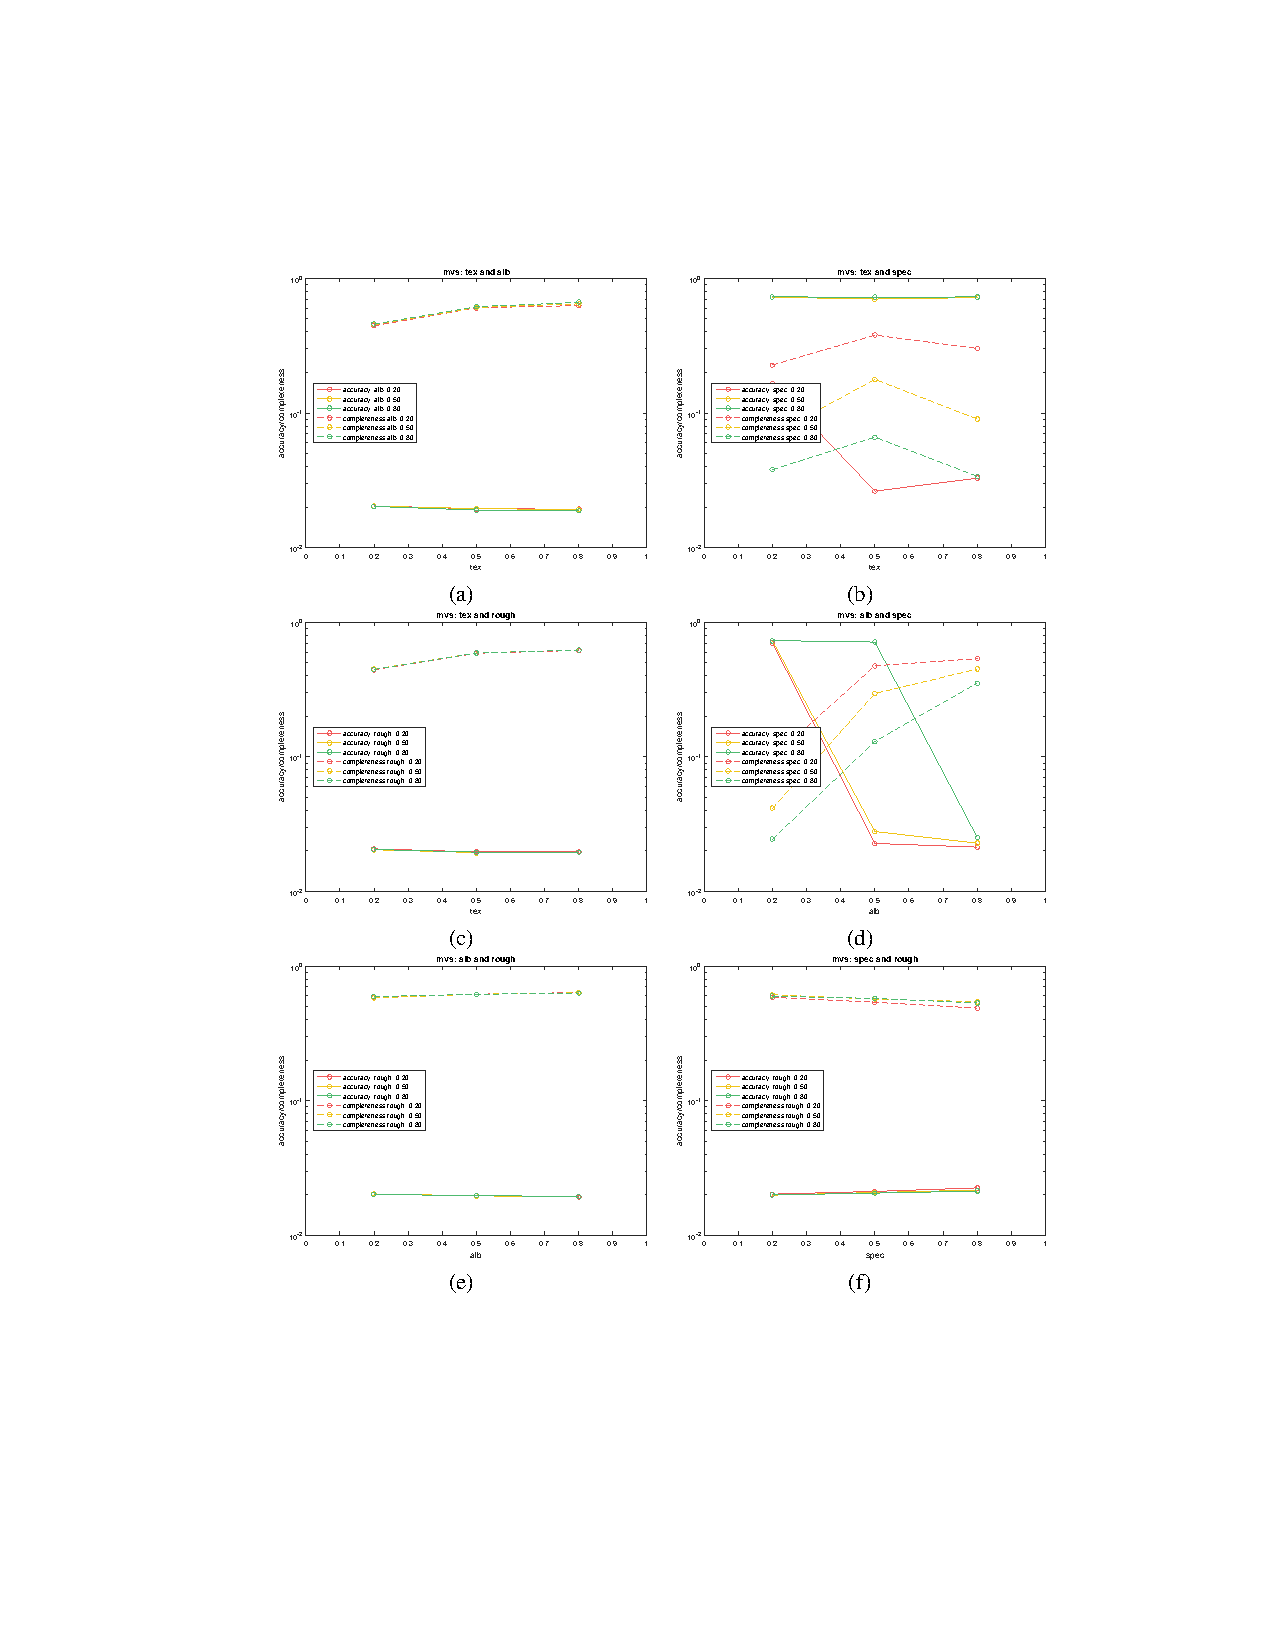
\includegraphics[width=\textwidth]{training/depend_check_mvs}
\caption{Performance of MVS with varied properties}
\label{fig:depend_check_mvs}
\end{figure}

\subsection{$C_1L_n-T-I-MDS-N$}
We evaluate the performance of PS in terms of angle difference under varied combinations of properties. The statistical measures that we used include median, mean, first and third quartile. We investigate two properties at a time.

\begin{table}[h]
  \centering
  \begin{tabular}{l*{5}{c}}
  \hline
  \textbf{Property} & Texture coverage & Albedo & Specular/Diffuse ratio & Roughness\\
  \hline
  \textit{Value} & 0.2-0.8 & 0.2-0.8 & 0.0 & 0.0\\
                 & 0.2-0.8 & 1 & 0.2-0.8 & 0.0\\
                 & 0.2-0.8 & 1 & 0.0 & 0.2-0.8\\
                 & 0.0 & 0.2-0.8 & 0.2-0.8 & 0.0\\
                 & 0.0 & 0.2-0.8 & 0.0 & 0.2-0.8\\
                 & 0.0 & 1.0 & 0.2-0.8 & 0.2-0.8\\
  \hline
  \end{tabular}
  \caption{Parameter of PS with varied properties}
\end{table}

\textbf{(a) Texture and Albedo} 
For a fixed texture, as the albedo level goes up, all the statistic measures go down, which means that the reconstruction gets better as albedo level goes up, which is consistent to the real-world scenario.

For a fixed albedo, the angle difference doesn't change much as the texture level changes, which shows that texture doesn't interfere with albedo, and these two properties are thus independent.

\textbf{(b) Texture and Specularity} 
For a fixed texture, as the specularity goes up, all the statistic measures go up, which means that the reconstruction gets worse as specularity level goes up, which is consistent to the real-world scenario.

For a fixed specularity, the angle difference doesn't change much as the texture level changes, which shows that texture doesn't interfere with specularity, and these two properties are independent.

\textbf{(c) Texture and Roughness} 
For a fixed texture, as the roughness goes up, all the statistic measures go down, which means that the reconstruction gets better as roughness level goes up.

For a fixed roughness, the angle difference doesn't change much as the texture level changes, which shows that texture doesn't interfere with roughness, and these two properties are independent.

\textbf{(d) Albedo and Specularity} 
We're using a physically-based renderer, thus the higher the specularity, the less the diffusion would be. Thus rising specularity would `darken' the diffuse areas.

For a fixed albedo, the angle difference goes up as the specularity rises, which demonstrate that PS can't deal with high specularity, and it's worse for lower albedo surfaces than that for the higher albedo surfaces, which is consistent to real-world scenario.

For a fixed specularity, the angle difference goes down as the albedo rises, which is consistent to the real-world scenario since high albedo would make the intensity variation more distinctive.

\textbf{(e) Albedo and Roughness} 
For a fixed albedo, as the roughness goes up, all the statistic measures go down, which means that the reconstruction gets better as roughness level goes up.

For a fixed roughness, the angle difference also goes down as the albedo level goes up, which shows that albedo does interfere with roughness, and these two properties are dependent.

\textbf{(f) Specularity and Roughness}
For a fixed specularity, if the specularity is lower, the effect of roughness is less noticeable, whereas if the specularity is higher, the effect of roughness becomes more substantial. We've also noticed a `peculiar' case when roughness is 0.5, it makes the reconstruction worse, which is counter-intuitive. However, we argue that it's because the roughness effect is not strong enough to cancel out the specularity, thus causing a much larger area of `blurred' specularity, which makes the reconstruction worse. This effect is also demonstrated in the training stage, see Figure~\ref{fig:ps_outlier} for some visual examples.

For a fixed roughness, increasing the specularity would make the angle difference worse. The effect is less substantial when the roughness is higher or when the specularity is lower.

Therefore, the specularity and roughness cancels each other's effect, thus they are dependent properties, which is consistent to visual inspection.

\textbf{Conclusion} the properties that have an effect on the PS are: albedo, specularity, and roughness. Therefore, we will only consider these three properties for all forthcoming discussion of PS.

\begin{figure}[h!]
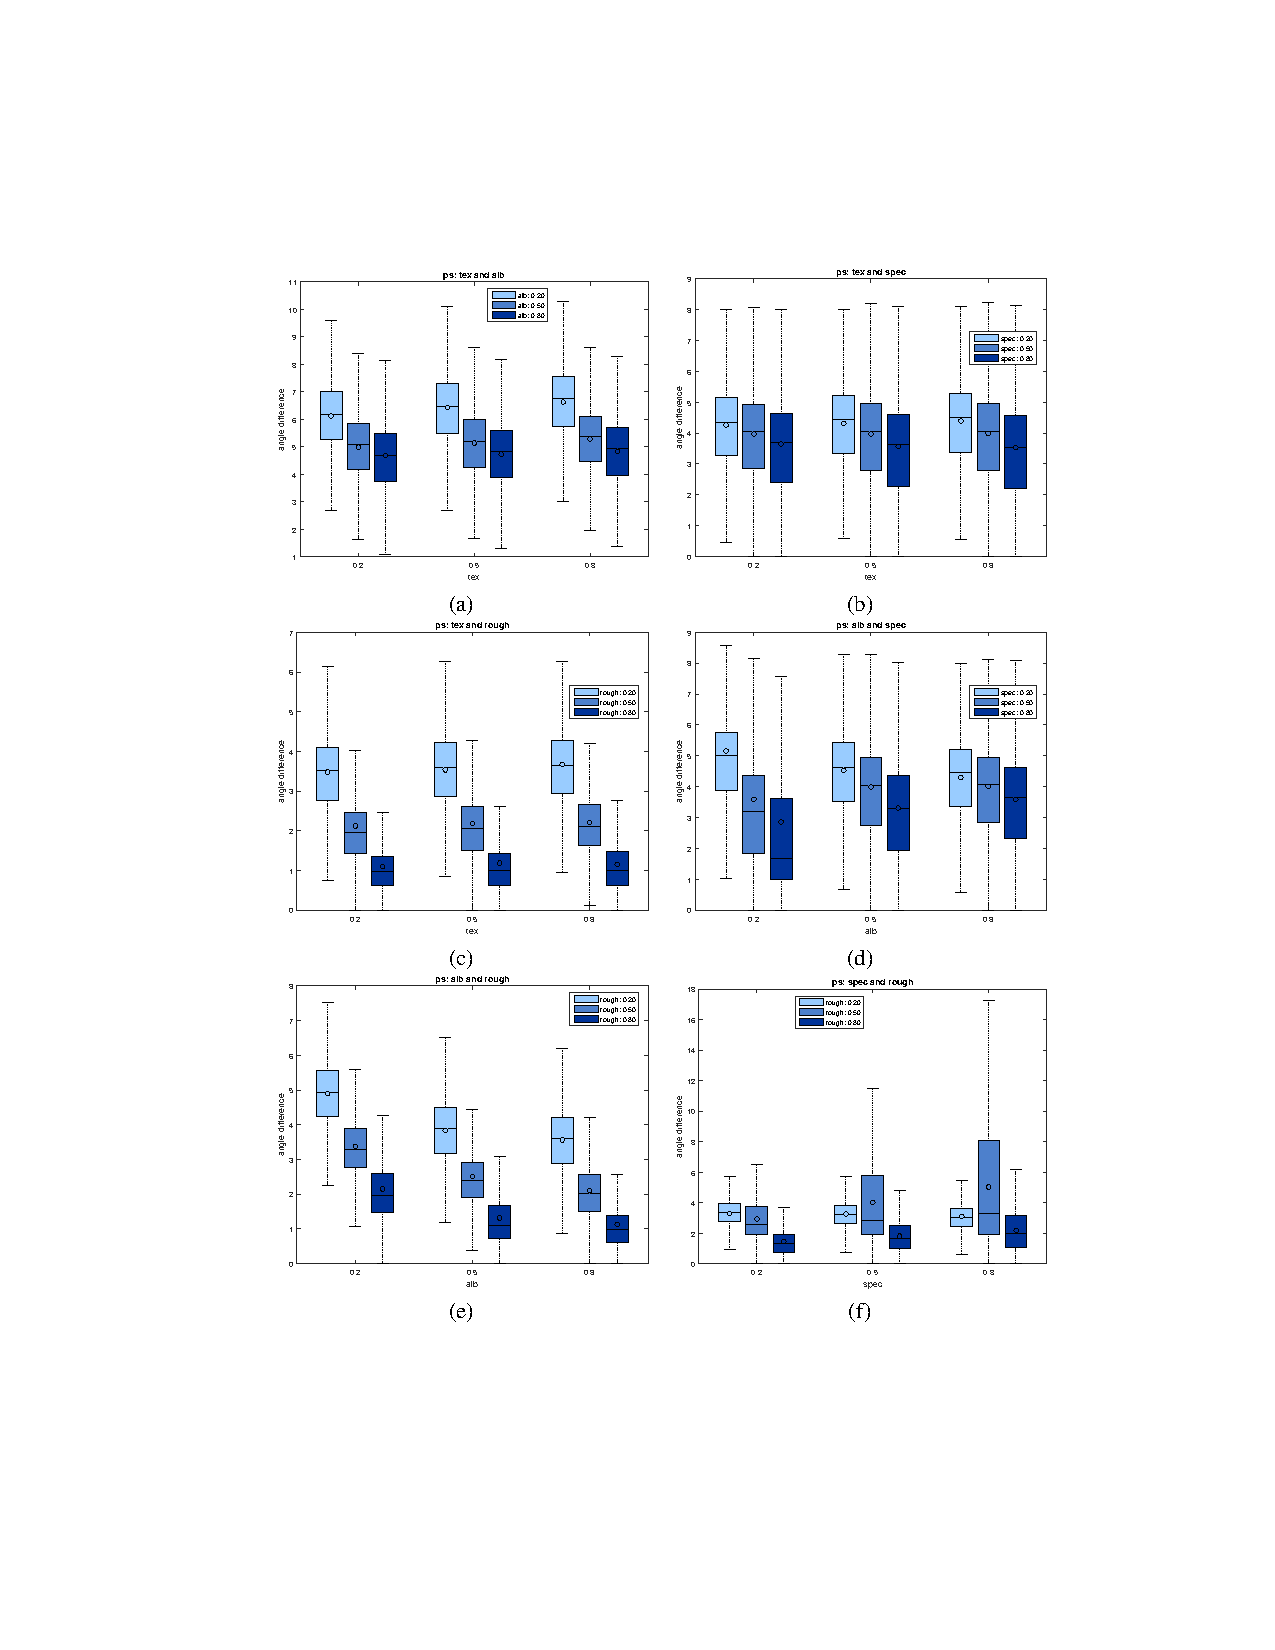
\includegraphics[width=\textwidth]{training/depend_check_ps}
\caption{Performance of PS with varied properties}
\label{fig:depend_check_ps}
\end{figure}

\subsection{$C_1P-T-I-B-P$}
We evaluate the performance of SL in terms of accuracy and completeness under varied combination of properties.

\begin{table}[h]
  \centering
  \begin{tabular}{l*{5}{c}}
  \hline
  \textbf{Property} & Texture coverage & Albedo & Specular/Diffuse ratio & Roughness\\
  \hline
  \textit{Value} & 0.2-0.8 & 0.2-0.8 & 0.0 & 0.0\\
                 & 0.2-0.8 & 1 & 0.2-0.8 & 0.0\\
                 & 0.2-0.8 & 1 & 0.0 & 0.2-0.8\\
                 & 0.0 & 0.2-0.8 & 0.2-0.8 & 0.0\\
                 & 0.0 & 0.2-0.8 & 0.0 & 0.2-0.8\\
                 & 0.0 & 1.0 & 0.2-0.8 & 0.2-0.8\\
  \hline
  \end{tabular}
  \caption{Parameter of SL with varied properties}
\end{table}

Our current implementation of SL projects column patterns and a row patterns, and compute depth values using images captured using these two kinds of patterns individually. A depth consistency checking step is performed to reject erreneous triangulations, thus the accuracy remains almost the same across all cases.

\textbf{(a) Texture and Albedo} 
For a fixed texture, as the albedo goes up, the accuracy value of SL remain almost the same, whereas the completeness goes up, meaning that the reconstruction gets more dense as albedo goes up, which is consistent to real-world scenario.

For a fixed albedo, the accuracy remains almost the same as the texture level goes up, and the completeness goes down a little as the texture goes up, which demonstrate the real-world observation that surface texture would interfere with some SL techniques.

\textbf{(b) Texture and Specularity} 
No substantial changes when either of the two properties changes.

\textbf{(c) Texture and Roughness} 
No substantial changes when either of the two properties changes.

\textbf{(d) Albedo and Specularity} 
For a fixed albedo, the completeness goes down as the specularity goes up for low albedo surface, this effect becomes less when the albedo increases. Thus these two properties are dependent

\textbf{(e) Albedo and Roughness} 
No substantial changes when either of the two properties changes.

\textbf{(f) Specularity and Roughness} 
No substantial changes when either of the two properties changes.

\textbf{Conclusion} the properties that have an effect on the SL are: texture, albedo, specularity. Therefore, we will only consider these three properties for all forthcoming discussion of SL.

\begin{figure}[h!]
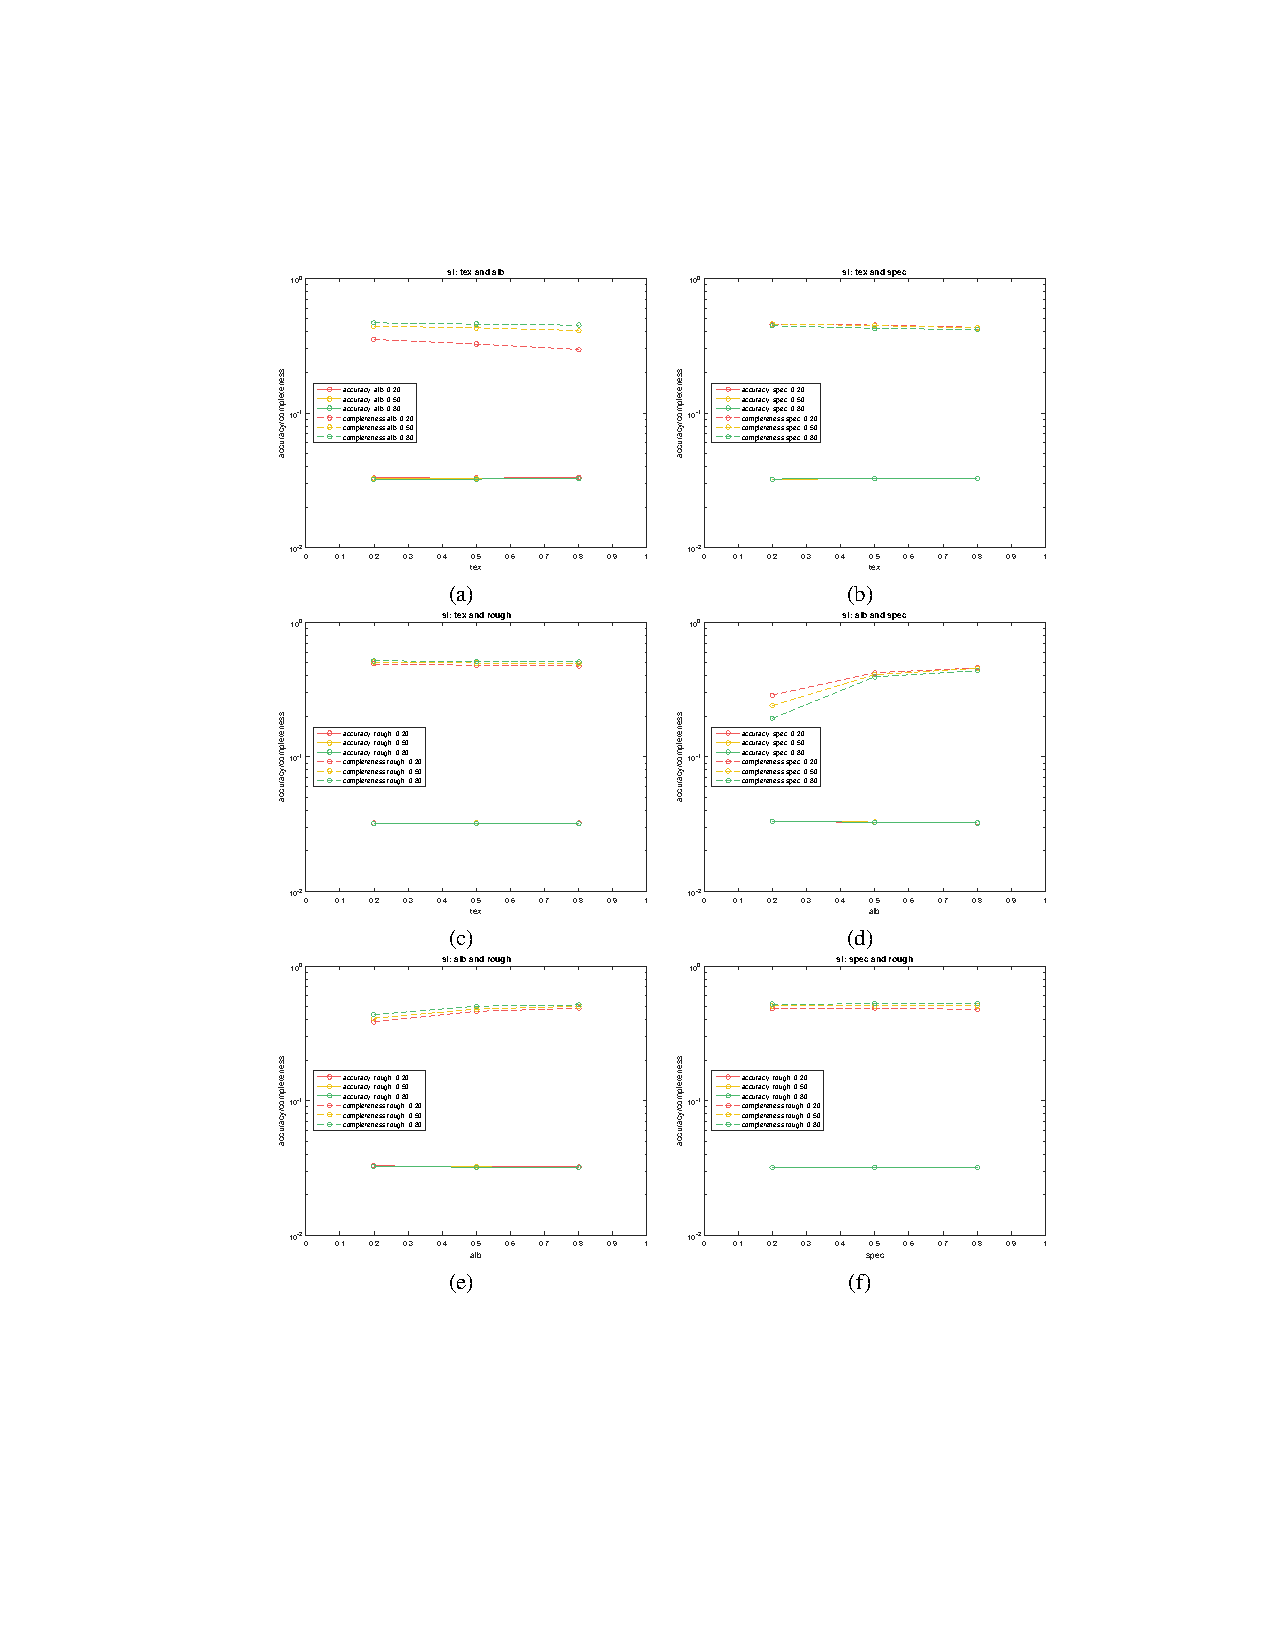
\includegraphics[width=\textwidth]{training/depend_check_sl}
\caption{Performance of SL with varied properties}
\label{fig:depend_check_sl}
\end{figure}

\section{Training}
For each technique, we generate the synthetic dataset using only the dependent properties, thus there are $L\times L\times L$ different combinations for each technique, where $L$ is the number of levels for each property. We show the performance of each technique w.r.t one property in Figure~\ref{fig:training}, note that column 2, 3 uses the exactly same data as column 1.

\begin{figure}[h!]
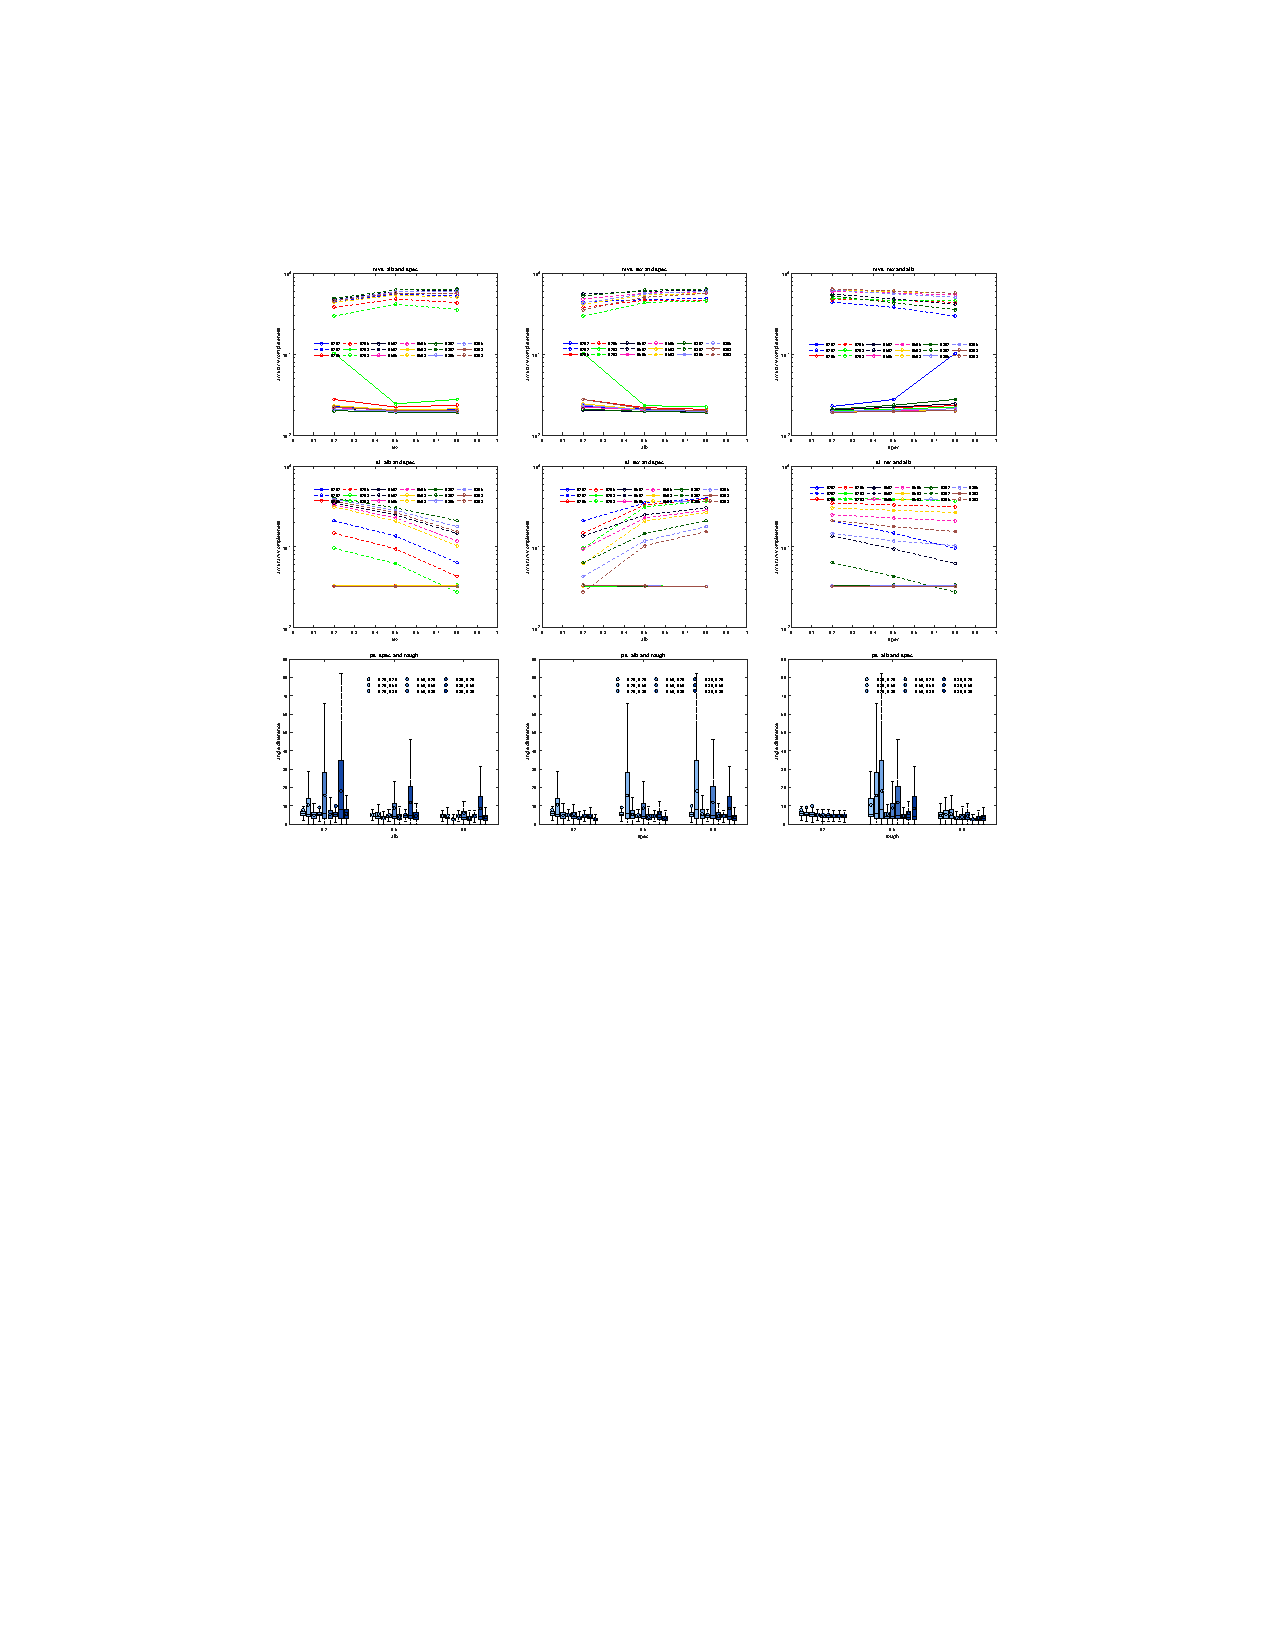
\includegraphics[width=\textwidth]{training/training}
\caption{Performance of MVS, SL and PS with varied properties. Each each column, we fix one property while changing the others, thus the second and the third columns are essentially the same as the first column, they are just different point of views of looking at those relations. Each line/boxplot represents a different combinations of property values: 0202, 0205, 0208, 0502, ..., 0808. Beware that we consider \{tex, alb, spec\} for MVS and SL, and \{alb, spec, rough\} for SL.}
\label{fig:training}
\end{figure}

\section{Summary}

